%==============================================================================
% CAPITOLUL 3 - Implementarea functionalitatilor si punerea in functiune
% Varianta finala: fara cod (cod in Anexe), include sectiune noua despre indoor.
%==============================================================================

\chapter{Implementarea funcționalităților și punerea în funcțiune}
\label{cap:implementare}

După descrierea fundamentelor teoretice și a arhitecturii sistemului, acest
capitol arată cum funcționează platforma în practică. Sunt prezentate, pe rând,
gestionarea rolurilor de utilizator, editarea hărții de către administrator,
căutarea și afișarea informațiilor, măsurile de securitate la nivelul
interfeței, rutarea exterioară cu afișarea vizuală a traseului, rutarea în
interiorul clădirilor și, la final, infrastructura de rețea care face platforma
accesibilă în condiții de siguranță. Fragmentele de cod sunt grupate în Anexa~A
(backend) și Anexa~B (frontend), iar în text se face trimitere la ele acolo
unde este cazul.

\section{Gestionarea rolurilor și modurile de utilizare}
\label{sec:roluri-impl}

Platforma distinge două categorii de utilizatori, fiecare cu un mod propriu de
interacțiune. Utilizatorii obișnuiți au acces în mod de vizualizare: pot
explora harta, căuta clădiri și săli, consulta informații și calcula trasee.
Administratorii au în plus un mod de editare, prin care pot modifica structura
hărții campusului. Diferențierea este aplicată la nivelul backend-ului, prin
mecanismul de securitate descris în capitolul anterior, astfel încât accesul la
funcțiile de editare nu poate fi obținut din interfața clientului fără
autentificarea corespunzătoare.

După autentificare, rolul utilizatorului determină cum este încărcată
interfața. Pentru un administrator sunt activate controalele de editare, în
timp ce pentru un utilizator obișnuit acestea rămân ascunse, interfața fiind
orientată exclusiv spre consultare și navigare. Separarea celor două
experiențe protejează datele împotriva modificărilor neautorizate și păstrează
interfața curată pentru fiecare categorie de utilizatori.

% [CAPTURA 3.1: mod vizualizare vs mod editare]

\section{Editarea hărții de către administrator}
\label{sec:editare-impl}

Una dintre funcționalitățile centrale ale platformei este posibilitatea
administratorului de a edita structura hărții direct din interfață. În modul
de editare, administratorul poate defini și modifica rețeaua de noduri și
muchii pe care se bazează rutarea, adăugând puncte de traseu, legături între
ele și elemente de infrastructură relevante pentru navigare. Această
capabilitate este esențială pentru mentenabilitatea sistemului: actualizarea
hărții se face vizual, prin interacțiune directă cu harta, fără intervenții în
cod sau în baza de date.

Modificările efectuate de administrator sunt transmise către backend prin
serviciile dedicate gestionării grafului și sunt persistate în baza de date.
Structura hărții, serializată în format JSON, este actualizată în entitatea
corespunzătoare și devine imediat disponibilă tuturor utilizatorilor la
accesările ulterioare. O modificare făcută de un administrator, adăugarea
unui traseu nou sau corectarea unei legături, se reflectă în mod centralizat,
fără a fi nevoie de redistribuirea aplicației.

Într-un campus universitar, infrastructura se modifică în timp: apar săli noi,
unele se închid pentru lucrări, denumirile clădirilor pot fi actualizate.
Capacitatea de a întreține harta rapid, fără efort tehnic, asigură că
platforma rămâne utilă pe termen lung.

\begin{figure}[H]
    \centering
    \begin{subfigure}[b]{0.40\textwidth}
        \centering
        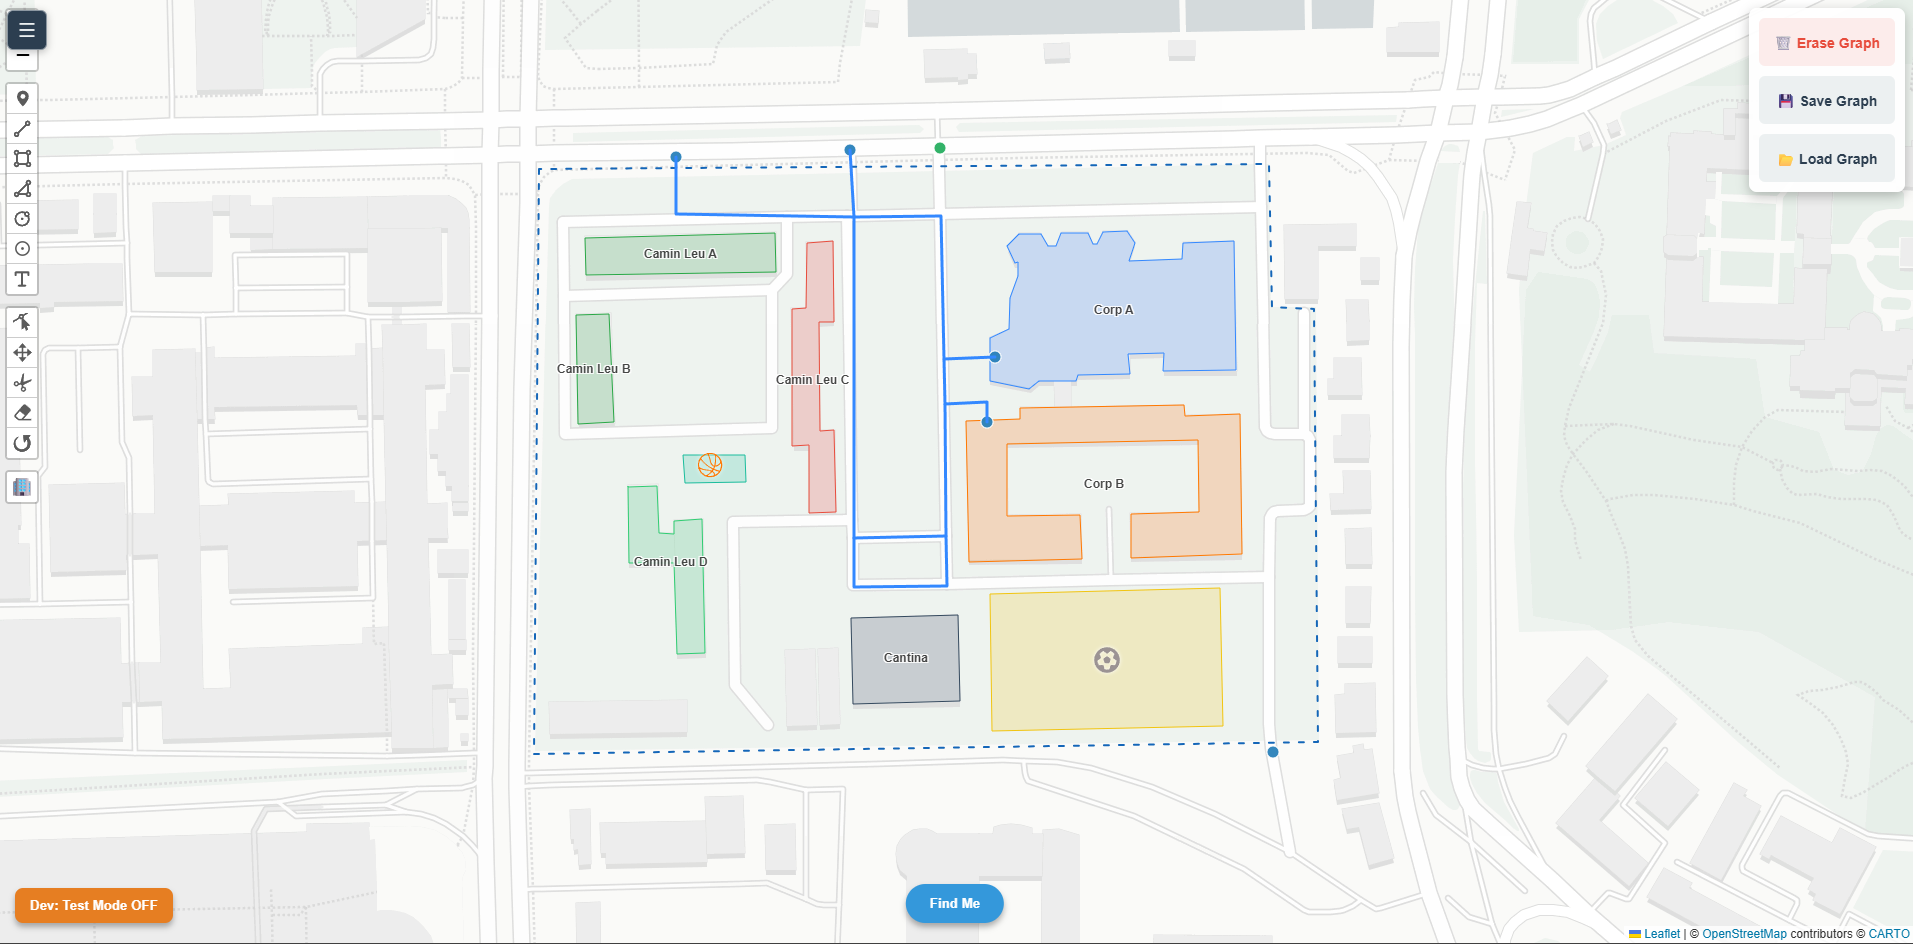
\includegraphics[width=\textwidth]{figuri/harta-edit.png}
        \caption{Modul de editare al harții}
        \label{fig:edit-cam}
    \end{subfigure}
    \hfill
    \begin{subfigure}[b]{0.40\textwidth}
        \centering
        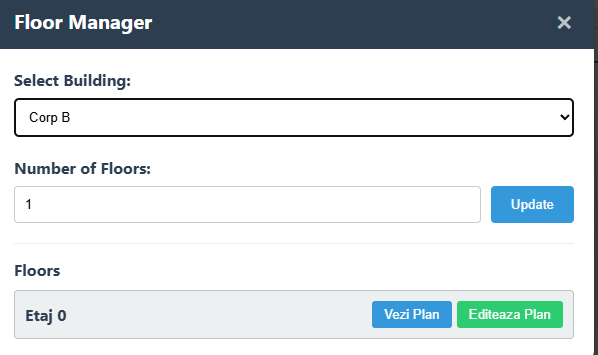
\includegraphics[width=\textwidth]{figuri/manager-etaje.png}
        \caption{Managerul de etaje interioare}
        \label{fig:edit-mark}
    \end{subfigure}
    \hfill
    \begin{subfigure}[b]{0.40\textwidth}
        \centering
        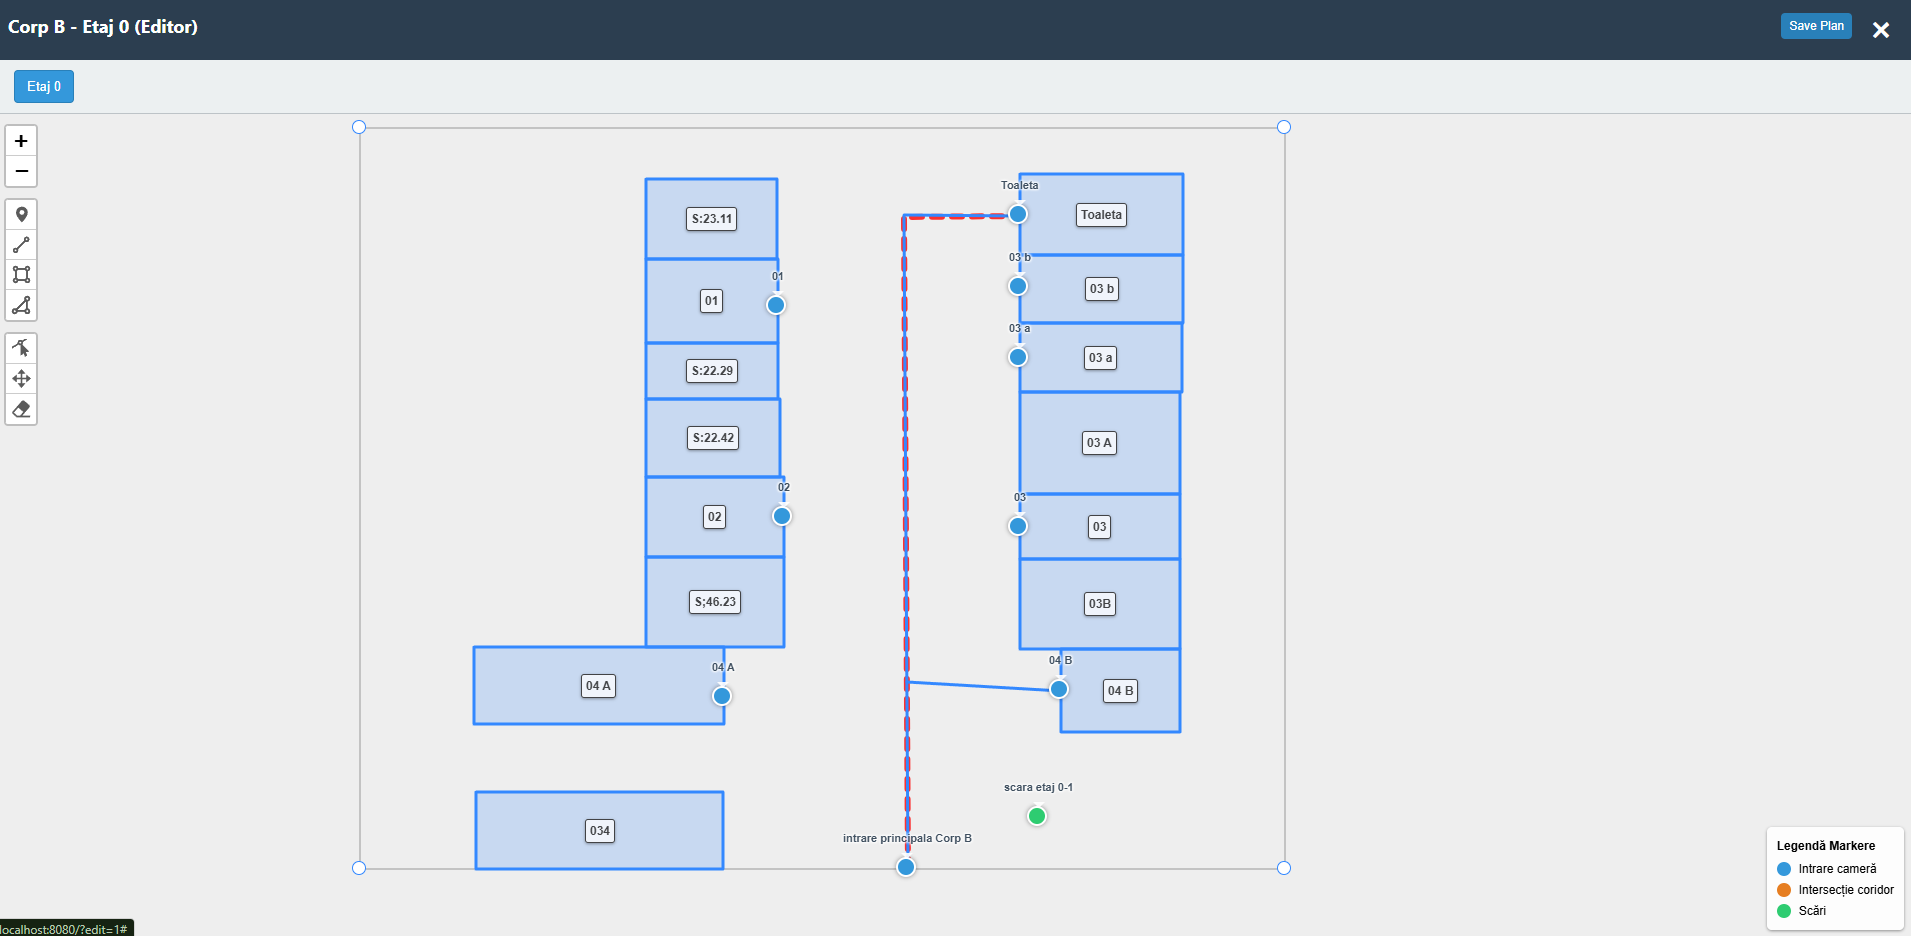
\includegraphics[width=\textwidth]{figuri/editare-etaje.png}
        \caption{Modul de editare al planului per etaj}
        \label{fig:edit-save}
    \end{subfigure}
    \caption{Fluxul de editare în modul administrator}
    \label{fig:edit-flow}
\end{figure}

% [CAPTURA 3.2: admin editand harta]

\section{Căutarea și afișarea informațiilor}
\label{sec:cautare-impl}

Pentru a permite utilizatorilor să localizeze rapid o sală sau o clădire,
platforma include o funcție de căutare integrată în panoul lateral. Căutarea
acoperă atât clădirile exterioare, cât și camerele din planurile de etaj
indoor, oferind rezultate unificate indiferent de natura locației. Utilizatorul
introduce un termen de căutare, iar aplicația identifică elementele
corespunzătoare și le afișează, permițând selectarea celui dorit. Pentru
utilizatorii nefamiliarizați cu infrastructura campusului, această funcție
reduce semnificativ timpul de orientare.

La selectarea unui element, aplicația afișează detaliile asociate. Pentru o
sală, sunt prezentate clădirea în care se află, etajul, capacitatea și tipul,
însoțite, atunci când există, de o descriere suplimentară. Detaliile sunt
generate dinamic și apar fie într-un panou dedicat, fie într-o fereastră de
tip popup atașată locației pe hartă, în funcție de contextul interacțiunii.
Aceeași logică de generare produce ambele variante, parametrizată după
context, ceea ce evită duplicarea codului și asigură consistența informației.

% [CAPTURA 3.3: cautare + detalii sala]

\section{Securitatea la nivelul interfeței}
\label{sec:securitate-frontend-impl}

Pe lângă mecanismele de securitate de la nivelul backend-ului, descrise în
capitolul anterior, platforma aplică măsuri de protecție și la nivelul
interfeței. O preocupare frecventă în aplicațiile web care afișează date este
prevenirea injectării de cod prin conținut nesigur, o categorie de
vulnerabilități cunoscută sub numele de cross-site scripting. Problema apare
când date provenite dintr-o sursă externă sunt inserate direct în pagină fără
prelucrare, ceea ce permite execuția unui cod neintenționat.

Pentru a preveni astfel de situații, valorile text, numele unei săli,
descrierea acesteia, sunt trecute, înainte de a fi inserate în pagină,
printr-o funcție de prelucrare care transformă caracterele speciale în
echivalente inofensive (vezi Listing~B.5 din Anexa~B). Orice conținut
potențial periculos este tratat ca text simplu, nu ca instrucțiuni
executabile. Tehnica folosită se bazează pe un mecanism oferit nativ de
browser: textul este atribuit unui element printr-o proprietate care îl
tratează exclusiv ca text, iar apoi este extras în forma sa deja
neutralizată. Soluția este simplă, dar suficientă pentru scenariul de față,
și contribuie la robustețea generală a platformei.

\section{Rutarea exterioară și afișarea vizuală a traseului}
\label{sec:rutare-exterior}

Rutarea exterioară reunește componentele descrise în capitolul de arhitectură
într-o experiență vizuală completă. Utilizatorul selectează un punct de
plecare, care poate fi propria poziție obținută prin GPS, și un punct de
destinație, iar aplicația calculează și afișează traseul optim între acestea,
desenat direct pe hartă.

Procesul se desfășoară integral pe partea de client. Punctele alese sunt mai
întâi asociate celor mai apropiate noduri din graful de navigare, după care
algoritmul lui Dijkstra determină lanțul de noduri care formează drumul de
cost minim. Rezultatul, o secvență de coordonate, este apoi transformat
într-o linie trasată pe hartă, suprapusă peste infrastructura campusului,
oferind utilizatorului o reprezentare clară a traseului de urmat.

Afișarea vizuală a traseului transformă rezultatul abstract al unui algoritm
într-un ghid practic de orientare. Combinată cu poziționarea în timp real a
utilizatorului, această funcție permite navigarea efectivă prin campus: pe
măsură ce utilizatorul se deplasează, poziția sa este actualizată pe hartă,
raportată la traseul calculat. Atunci când nu există un traseu valid, de
exemplu între puncte aflate pe porțiuni neconectate ale rețelei, aplicația
informează utilizatorul în loc să afișeze un rezultat eronat.

% [CAPTURA 3.4: traseu exterior pe harta]

\section{Rutarea în interiorul clădirilor}
\label{sec:indoor}

O componentă importantă a platformei este rutarea în interiorul clădirilor,
care extinde experiența de navigare dincolo de granița porților de intrare.
Soluția adoptată urmează aceeași abordare ca rutarea exterioară: o rețea de
noduri și muchii pe care se aplică algoritmul lui Dijkstra. Diferența ține de
modul în care sunt achiziționate datele și de modul în care este reprezentată
poziția utilizatorului.

\subsection{Modelul de date al planurilor de etaj}
\label{subsec:indoor-model}

Fiecare etaj al unei clădiri are propriul plan, stocat ca un document GeoJSON
în câmpul \texttt{indoorJson} al entității \texttt{MapData} descrisă în
Capitolul~2. Planul conține trei
tipuri de elemente: camere (poligoane închise, cu nume), noduri (puncte de
decizie pe coridoare, de tip intrare în cameră, intersecție sau scară) și
muchii (linii care leagă două noduri și reprezintă un segment de coridor).
Această structură este consistentă cu modelul folosit pentru harta
exterioară, doar că lucrează pe un sistem de coordonate plan local, specific
fiecărui plan de etaj.

Asocierea dintre o cameră și rețeaua de coridoare se face prin nodul de
intrare: lângă fiecare ușă, administratorul plasează un nod de tip „intrare"
și îi asociază numele camerei. Astfel, o cameră devine rutabilă: pentru a
calcula traseul către ea, este suficient să se cunoască nodul ei de intrare.

\subsection{Editarea planurilor și salvarea în baza de date}
\label{subsec:indoor-editare}

Administratorul construiește planul unui etaj direct din interfață, folosind
uneltele de desen ale bibliotecii Leaflet.PM. Camerele sunt desenate ca
dreptunghiuri sau poligoane, iar la fiecare creare aplicația cere
administratorului numele camerei și îl atașează ca proprietate a formei.
Nodurile sunt plasate ca markeri, iar tipul lor, intrare, intersecție sau
scară, este ales tot printr-un dialog scurt la momentul plasării.
Coridoarele sunt desenate ca linii între noduri.

La salvare, întregul conținut al planului este serializat în GeoJSON și
trimis către backend printr-o cerere dedicată, care îl persistă în entitatea
\texttt{indoorJson} al entității \texttt{MapData}. La reîncărcare,
aplicația cere planul de pe server și îl restaurează vizual împreună cu toate
proprietățile. Acest ciclu complet de desenare, salvare și reîncărcare
funcționează autonom, fără ca administratorul să fie nevoit să exporte sau să
încarce manual fișiere.

% [CAPTURA 3.5: admin desenand un plan de etaj cu camere si coridoare]

\subsection{Calculul traseului indoor}
\label{subsec:indoor-rutare}

La nivel de utilizator obișnuit, fluxul de rutare indoor pornește de la
căutare. Atunci când utilizatorul caută o cameră, de exemplu „B127", și o
selectează, aplicația identifică automat clădirea și etajul corespunzător și
deschide planul respectiv. Aici intervine particularitatea cea mai vizibilă a
navigării în interior: GPS-ul nu poate fi folosit pentru a determina poziția
utilizatorului, întrucât semnalul satelitar este blocat sau distorsionat de
structurile clădirii. Această limitare a fost discutată teoretic în
Capitolul~1.

Soluția adoptată este selecția explicită a punctului de plecare. Utilizatorul
indică pe planul de etaj unde se află, fie un nod de intersecție pe coridor,
fie intrarea unei camere apropiate. Această abordare este folosită inclusiv
de aplicații consacrate precum Google Maps în interiorul centrelor comerciale
și clădirilor publice, fiind robustă tocmai pentru că nu introduce o precizie
artificială pe care tehnologia nu o poate susține. Odată selectat punctul de
plecare, aplicația construiește graful etajului din GeoJSON-ul stocat,
rulează algoritmul lui Dijkstra între nodul de plecare și nodul de intrare al
camerei destinație și desenează traseul rezultat pe plan.

Versiunea actuală tratează rutarea pe un singur etaj. Pentru deplasări între
etaje, ar fi necesare noduri de tip scară sau lift, conectate între etaje
prin muchii speciale care reprezintă tranziții verticale. Implementarea
acestei extinderi este pregătită la nivel de model de date, nodurile de tip
scară sunt deja prevăzute, dar conectarea lor între etaje rămâne o
dezvoltare ulterioară.

% [CAPTURA 3.6: traseu indoor calculat si afisat pe planul de etaj]

\section{Punerea în funcțiune prin rețea privată virtuală}
\label{sec:deployment-impl}

Dincolo de implementarea funcționalităților, o componentă importantă a
contribuției practice o reprezintă punerea în funcțiune a platformei într-un
mediu accesibil de pe dispozitivele mobile ale utilizatorilor. În timpul
dezvoltării, întreaga aplicație rulează pe o singură mașină, clientul și
serverul comunicând prin interfața de buclă locală (\textit{loopback}), la
adresa 127.0.0.1. Pentru a deveni utilizabilă în campus, aplicația trebuie
să fie accesibilă de pe alte dispozitive, fără a fi expusă riscurilor
asociate publicării directe pe internet.

\subsection{Rețeaua privată cu Tailscale}
\label{subsec:tailscale-impl}

Pentru ETTIway, am ales Tailscale \cite{Tailscale}, o rețea privată virtuală
construită peste protocolul de criptare WireGuard \cite{WireGuard}. Spre
deosebire de un VPN clasic, în care tot traficul trece printr-un server
central, Tailscale realizează o rețea de tip \textit{mesh}: dispozitivele
înrolate, serverul pe care rulează aplicația și telefoanele de pe care este
accesată, comunică direct între ele, printr-un tunel criptat punct-la-punct.
Fiecare dispozitiv primește o adresă privată stabilă, validă doar în
interiorul rețelei virtuale.

Avantajul principal al acestei abordări este că serverul nu are nicio adresă
publică și niciun port deschis către internet. În arhitectura clasică,
expunerea unui server presupune redirecționarea porturilor pe ruterul rețelei
locale și deschiderea acestora către internet, ceea ce face serverul vizibil
și potențial atacabil de oriunde în lume. La ETTIway, această expunere
este eliminată: serverul, împreună cu baza de date PostgreSQL care ascultă pe
portul 5432 și cu aplicația Spring Boot, rămâne accesibil exclusiv
dispozitivelor autentificate în rețeaua privată. Pentru un proiect
administrat de o singură persoană, această configurație reduce semnificativ
suprafața de atac.

% [CAPTURA 3.7: panou Tailscale cu dispozitivele inrolate]

\subsection{Adresarea prin MagicDNS}
\label{subsec:magicdns-impl}

Pentru a evita memorarea adreselor numerice din rețeaua privată, Tailscale
oferă un mecanism propriu de rezolvare a numelor, denumit MagicDNS. Acesta
atribuie fiecărui dispozitiv un nume ușor de reținut, sub forma unui
subdomeniu în spațiul \texttt{.ts.net}, valabil doar în interiorul rețelei.
Serverul ETTIway este accesat printr-un nume stabil, care rămâne neschimbat
indiferent de rețeaua din care se conectează dispozitivele.

\subsection{Criptarea HTTPS și accesul la GPS}
\label{subsec:https-impl}

Comunicarea dintre dispozitiv și server este criptată prin protocolul HTTPS,
folosind un certificat digital emis automat de Tailscale prin autoritatea
Let's Encrypt \cite{LetsEncrypt}, pentru numele \texttt{.ts.net} al
serverului. Nu este nevoie de un domeniu public sau de o adresă IP publică
proprie. Certificatul este recunoscut de browsere ca fiind valid, iar
gestionarea sa, emiterea și reînnoirea periodică, este preluată automat de
infrastructura Tailscale, ceea ce reduce la minimum efortul de administrare.

Criptarea HTTPS are aici și o consecință tehnică ce depășește simpla
protecție a datelor. Browserele moderne impun ca interfețele sensibile,
precum cea de geolocalizare folosită pentru obținerea poziției prin GPS
\cite{MDN_Geolocation}, să poată fi utilizate doar într-un context securizat
\cite{MDN_SecureContext}, adică numai peste o conexiune criptată HTTPS. Fără
o astfel de conexiune, codul JavaScript al aplicației nu ar putea solicita
poziția utilizatorului, iar funcționalitatea de localizare exterioară ar fi
indisponibilă. Aici se observă cum aceeași infrastructură care asigură
izolarea față de internet oferă, în același timp, certificatul HTTPS necesar
pentru accesul la GPS.

% [CAPTURA 3.8: telefon cu .ts.net + HTTPS + pozitia GPS pe harta]

\section{Concluziile capitolului}
\label{sec:concluzii-cap3-impl}

În acest capitol au fost prezentate implementarea funcționalităților
principale și punerea în funcțiune a platformei ETTIway. La nivelul
funcționalităților, au fost descrise gestionarea rolurilor de utilizator și
administrator, editarea hărții direct din interfață cu persistarea
modificărilor în baza de date, căutarea unificată a clădirilor și a camerelor
indoor, măsurile de securitate aplicate la nivelul interfeței pentru
prevenirea injectării de cod, rutarea exterioară cu afișarea vizuală a
traseului pe hartă și rutarea în interiorul clădirilor, bazată pe planuri de
etaj editate de administrator și pe selecția explicită a punctului de
plecare.

La nivelul infrastructurii, a fost prezentată abordarea bazată pe o rețea
privată virtuală construită cu Tailscale peste protocolul WireGuard, care
elimină expunerea serverului pe internetul public și asigură, prin
certificatul HTTPS emis automat, contextul securizat necesar accesului la
poziția GPS a utilizatorului. Aceste elemente transformă aplicația dintr-un
prototip local într-o platformă funcțională, sigură și ușor de administrat,
în care securitatea este obținută prin proiectare. Fragmentele de cod care
implementează aceste mecanisme sunt grupate în Anexele~A și~B, pentru
cititorul care dorește detaliile tehnice.
